首先让内核打印出二级分页机制下地址空间的大小:

\begin{figure}[H]
    \centering
    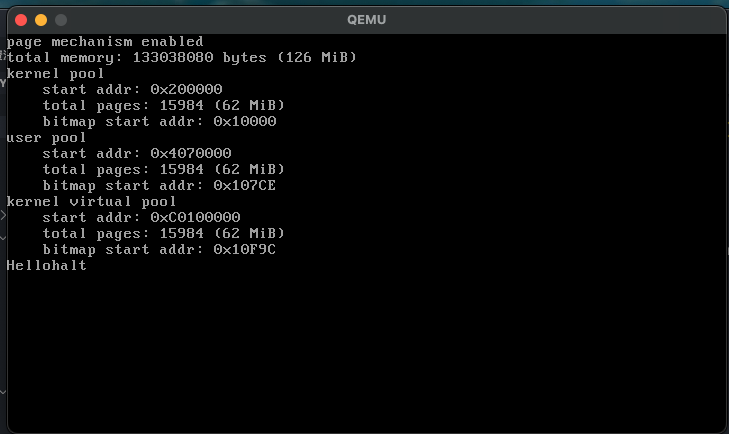
\includegraphics[width=\textwidth]{figures/page.png}
    \caption{三个地址空间}
    \label{fig:my_label}
\end{figure}

可以发现分页机制开启正常.

为了验证worst-fit算法,构造如下线程:
通过内存分配与释放得到两个大小分别为1页和80页的空隙,在此基础上申请一页内存,理论上这一页内存会从80页的空隙中分配.

\begin{figure}[H]
    \centering
    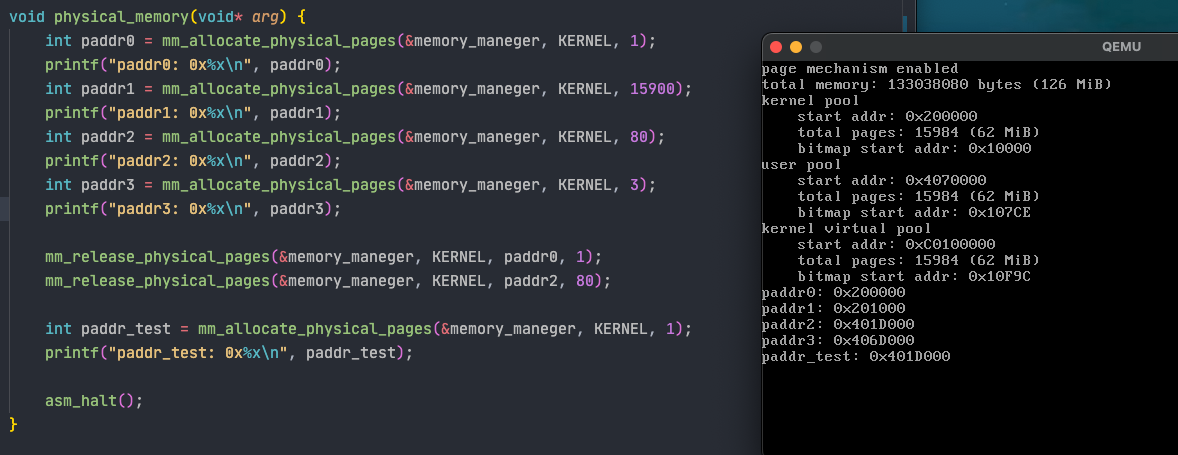
\includegraphics[width=\textwidth]{figures/wf_res.png}
    \caption{worst-fit算法验证代码与结果}
    \label{fig:my_label}
\end{figure}

可以看出,新的内存分配到了顺序上更后但更大的空隙中,算法完成.

为了验证FIFO算法,构造以下线程:
申请所有页之后,再次提出两个为4页的内存申请.理论上新的内存会获得最先进入的第0-7页.

\begin{figure}[H]
    \centering
    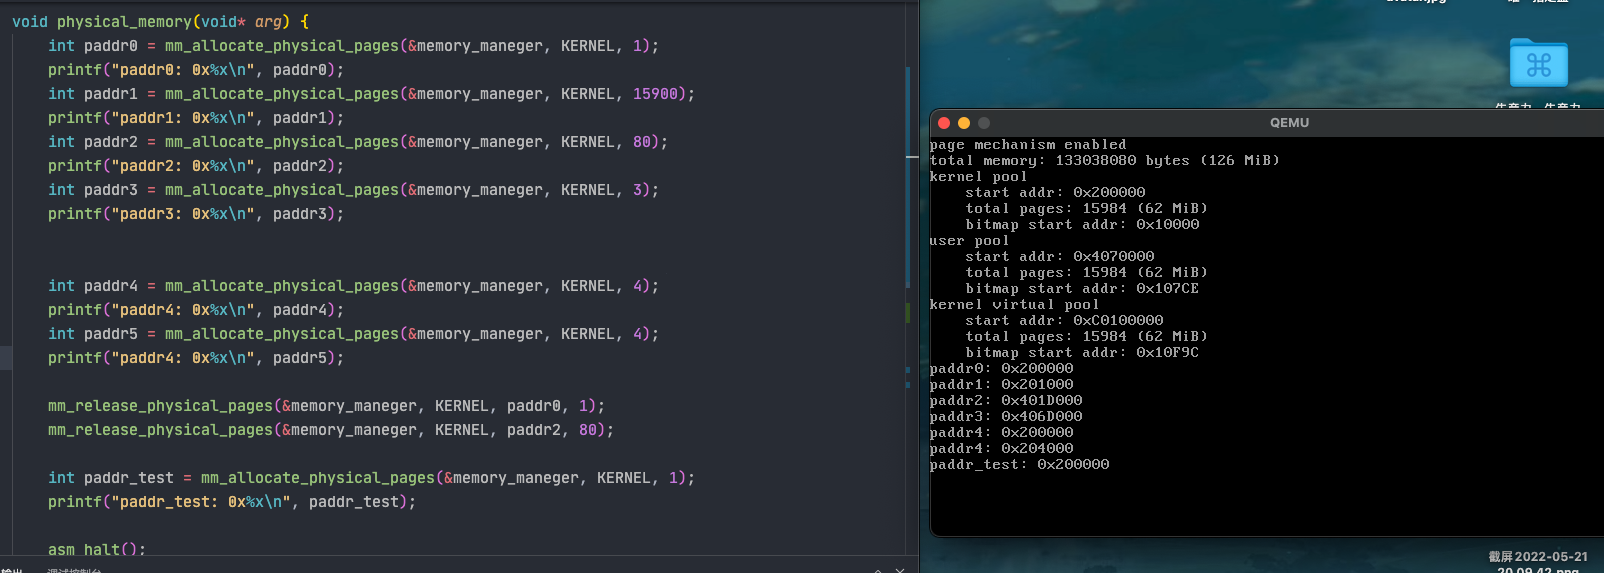
\includegraphics[width=\textwidth]{figures/fifo_res.png}
    \caption{FIFO算法验证代码与结果}
    \label{fig:my_label}
\end{figure}

可以看出,新的内存取代了最先分配的内存.

为了验证虚拟内存机制,构造以下线程:
申请三个虚拟内存页,打印出虚拟地址和物理地址,将其中一个页释放,再次申请一个内存页.理论上新内存的虚拟地址会跟在前三个后面,而物理地址将会与之前被释放的内存一样.

\begin{figure}[H]
    \centering
    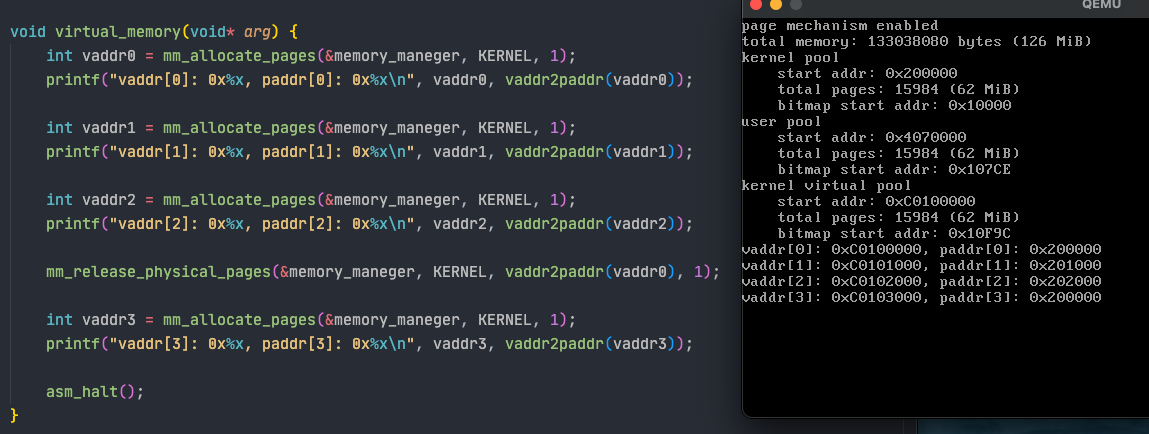
\includegraphics[width=\textwidth]{figures/vt_res.png}
    \caption{虚拟内存机制验证代码与结果}
    \label{fig:my_label}
\end{figure}

结果与预期一致.